\begin{frame}{비밀번호 제작(20304)}

\tiny

\begin{block}{문제}
서강대학교 전산실에서 보안직원으로 일하는 향빈이는 한 통의 이메일을 받게 되었다. 이메일에는 서버 관리자 계정에 대한 비정상적인 로그인 시도가 감지되었다는 내용이 적혀 있었고, 첨부된 파일에는 지금까지 로그인 시도에 사용된 비밀번호 목록이 있었다. 참고로, 서버 관리자 계정의 비밀번호로는 $0$ 이상 $N$ 이하의 정수 중 하나를 사용할 수 있다.

두 비밀번호의 안전 거리는 이진법으로 표현한 두 비밀번호의 서로 다른 자리의 개수로 정의한다. 예를 들어 $3$을 이진법으로 표현하면 $0011$, $8$을 이진법으로 표현하면 $1000$이 되고, 이때 서로 다른 자리의 개수는 $3$개이므로 $3$과 $8$의 안전 거리는 $3$이 된다.

어떤 비밀번호의 안전도는 지금까지 로그인 시도에 사용된 모든 비밀번호와의 안전 거리 중 최솟값으로 정의한다. 예를 들어 지금까지 로그인 시도에 사용된 비밀번호가 $3$과 $4$이라고 가정하면, 새로운 비밀번호 $8$에 대해 $3$과 $8$의 안전 거리는 $3$, $4$와 $8$의 안전 거리는 $2$이므로 비밀번호 $8$의 안전도는 $2$가 된다.

향빈이는 해커가 비밀번호를 알아내기까지의 시간을 최대한 늦추기 위해 현재 사용 중인 관리자 계정 비밀번호의 안전도가 가장 높게끔 바꾸고 싶다. 이때, 안전도가 제일 높은 비밀번호의 안전도를 구하여라.
\end{block}

\begin{block}{입력}
첫째 줄에 관리자 계정 비밀번호의 최댓값을 나타내는 정수 $N$이 주어진다. ($0 \leq N \leq 1\,000\,000$)

둘째 줄에는 로그인 시도에 사용된 비밀번호의 개수를 나타내는 정수 $M$이 주어진다. ($1 \leq M \leq 100\,000$)

셋째 줄에는 로그인 시도에 사용된 비밀번호 값인 정수 $p_1, p_2, \cdots, p_M$이 주어진다. ($0 \leq p_i \leq N$)
\end{block}

\begin{block}{출력}
안전도가 제일 높은 비밀번호의 안전도를 출력한다.
\end{block}

\end{frame}

\begin{frame}{가상의 정점 $S$를 추가한 Multi-source BFS}

\centering

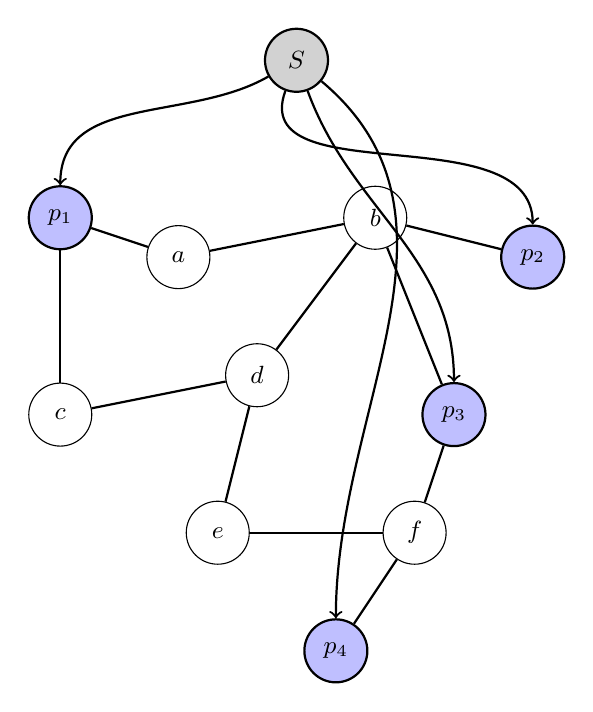
\begin{tikzpicture}[
    vertex/.style={
        circle,
        draw,
        minimum size=8mm,
        font=\small
    },
    source/.style={
        vertex,
        fill=blue!25,
        thick
    },
    supersource/.style={
        vertex,
        fill=gray!35,
        thick
    },
    sedge/.style={
        ->,
        thick
    },
    uedge/.style={
        thick
    },
    every node/.style={vertex}
]

% super source
\node[supersource] (S) at (0,3) {$S$};

% graph nodes
\node[source] (P1) at (-3,1) {$p_1$};
\node (A) at (-1.5,0.5) {$a$};
\node (B) at (1,1) {$b$};
\node[source] (P2) at (3,0.5) {$p_2$};

\node (C) at (-3,-1.5) {$c$};
\node (D) at (-0.5,-1) {$d$};
\node[source] (P3) at (2,-1.5) {$p_3$};

\node (E) at (-1,-3) {$e$};
\node (F) at (1.5,-3) {$f$};

\node[source] (P4) at (0.5,-4.5) {$p_4$};

% super source edges (directed, curved)
\draw[sedge] (S) to[out=210,in=90] (P1);
\draw[sedge] (S) to[out=250,in=90] (P2);
\draw[sedge] (S) to[out=290,in=90] (P3);
\draw[sedge] (S) to[out=320,in=90] (P4);

% undirected graph edges
\draw[uedge] (P1) -- (A);
\draw[uedge] (A) -- (B);
\draw[uedge] (B) -- (P2);

\draw[uedge] (P1) -- (C);
\draw[uedge] (C) -- (D);
\draw[uedge] (D) -- (B);

\draw[uedge] (B) -- (P3);
\draw[uedge] (D) -- (E);
\draw[uedge] (E) -- (F);

\draw[uedge] (P3) -- (F);
\draw[uedge] (F) -- (P4);

\end{tikzpicture}

\end{frame}

\setproblem{20304}

\begin{frame}[fragile, allowframebreaks]{원찬혁1 소스 코드}
\inputminted{java}{\prob/Chanhyeok1.java}
\end{frame}

\begin{frame}[fragile, allowframebreaks]{원찬혁2 소스 코드}
\inputminted{java}{\prob/Chanhyeok2.java}
\end{frame}

\begin{frame}[fragile, allowframebreaks]{김시온 소스 코드}
\inputminted{java}{\prob/Sion.java}
\end{frame}
